\documentclass[tikz,border=3.14mm]{standalone}
\usepackage{tikz}
\usetikzlibrary{shapes,arrows,positioning,calc}

\begin{document}
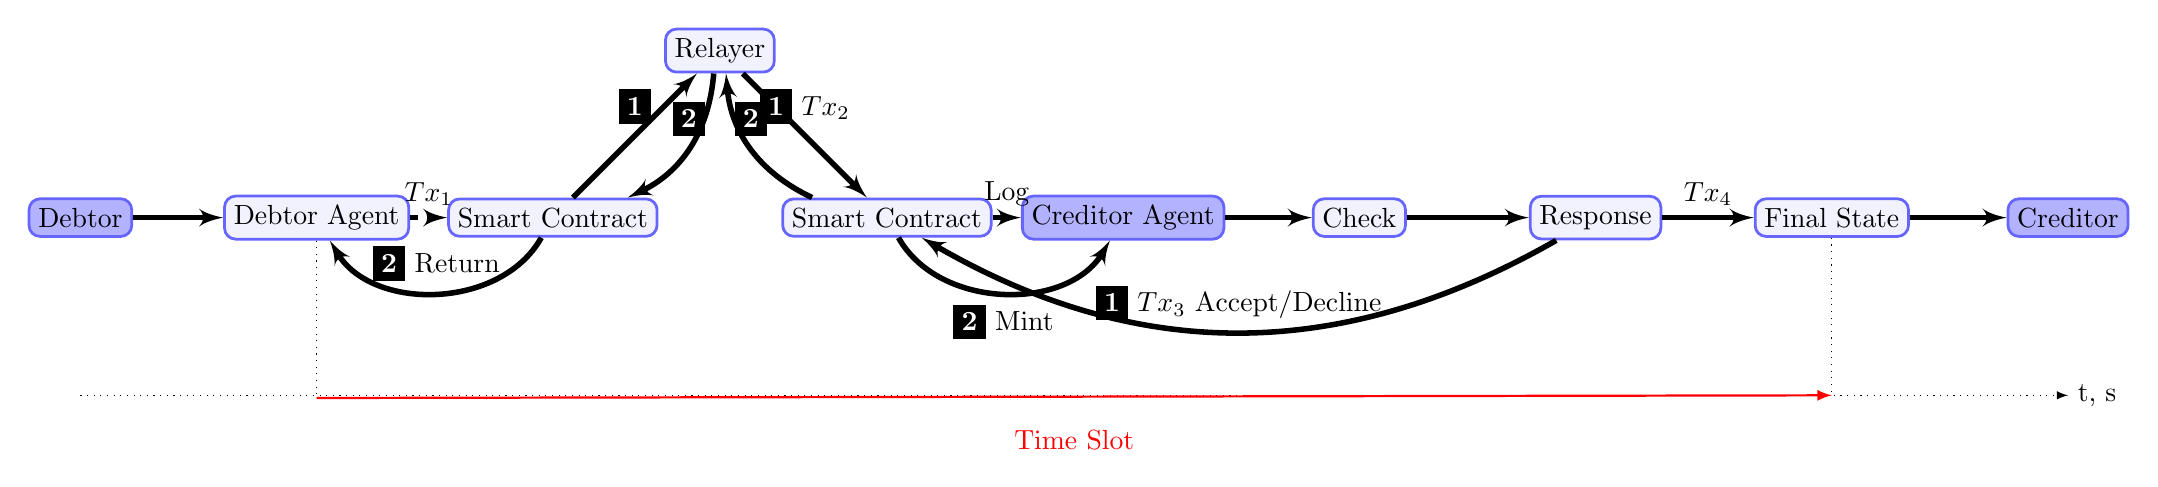
\begin{tikzpicture}[
    block/.style={rectangle, rounded corners, draw=blue!60, fill=blue!5, line width=1pt},
    blockfill/.style={rectangle, rounded corners, draw=blue!60, fill=blue!30, line width=1pt},
    line/.style={draw, -latex', line width=2pt},
    node distance=3cm
]

% Nodes
\node[blockfill] (debtor) {Debtor};
\node[block, right of=debtor] (debtoragent) {Debtor Agent};
\node[block, right of=debtoragent] (smartcontract) {Smart Contract};
\node[block, above right of=smartcontract] (relayer) {Relayer};
\node[block, below right of=relayer] (smartcontract2) {Smart Contract};
\node[blockfill, right of=smartcontract2] (creditoragent) {Creditor Agent};
\node[block, right of=creditoragent] (check) {Check};
\node[block, right of=check] (response) {Response};
\node[block, right of=response] (final) {Final State};
\node[blockfill, right of=final] (creditor) {Creditor};

% Lines
\draw[line] (debtor) -- (debtoragent);
\draw[line, dashed] (debtoragent) -- node[above] {$Tx_1$} (smartcontract);
% \draw[line, dashed] (smartcontract) -- node[above] {Response} (creditoragent);
  \draw[line,dashed] (smartcontract2) -- node[above] {Log} (creditoragent);
\draw[line] (creditoragent) -- (check);
\draw[line] (check) -- (response);
  \draw[line] (response) -- node[above] {$Tx_4$} (final);
\draw[line] (final) -- (creditor);

% Curved lines
  \draw[line] (response) to [bend left=30] node[midway,above] {\colorbox{black}{\textcolor{white}{\textbf{1}}} $Tx_3$ Accept/Decline} (smartcontract2);
  \draw[line] (smartcontract) to [bend left=60] node[midway,above] {\colorbox{black}{\textcolor{white}{\textbf{2}}} Return} (debtoragent);
  \draw[line] (smartcontract2) to [bend right=60] node[midway,below] {\colorbox{black}{\textcolor{white}{\textbf{2}}} Mint} (creditoragent);

% Lines to and from Relayer
  \draw[line] (smartcontract) -- node[midway,above] {\colorbox{black}{\textcolor{white}{\textbf{1}}}} (relayer);
  \draw[line] (relayer) -- node[midway,above] {\colorbox{black}{\textcolor{white}{\textbf{1}}} $Tx_2$} (smartcontract2);
  \draw[line] (smartcontract2) to [bend left=30] node[midway,above] {\colorbox{black}{\textcolor{white}{\textbf{2}}}} (relayer);
  \draw[line] (relayer) to [bend left=30] node[midway,above] {\colorbox{black}{\textcolor{white}{\textbf{2}}}} (smartcontract);

% Define timeline
\coordinate (timeline_start) at ([yshift=-2cm]debtor.south);
\coordinate (timeline_end) at ([yshift=-2cm]creditor.south);
\draw[dotted, -latex] (timeline_start) -- (timeline_end) node[right] {t, s};

% Define marked period
\coordinate (marked_start) at ([yshift=-2cm]debtoragent.south);
\coordinate (marked_end) at ([yshift=-2cm]final.south);
\draw[thick, red, -latex] (marked_start) -- (marked_end) node[midway, below=3mm] {Time Slot};

% Connect marked period with flowchart
\draw [dotted] (debtoragent.south) -- (marked_start);
\draw [dotted] (final.south) -- (marked_end);

\end{tikzpicture}
\end{document}
